\documentclass[tikz,border=4pt]{standalone}
\usepackage{tgadventor}
\usepackage{tgheros}
\usepackage{graphicx}
\usepackage{xcolor}
\usepackage{tikz}
\usetikzlibrary{arrows.meta,calc}
\newcommand{\headingfont}{\fontfamily{qag}\selectfont}
\newcommand{\bodyfont}{\fontfamily{qhv}\selectfont}
\renewcommand{\familydefault}{qhv}
\definecolor{orange}{RGB}{245,118,20}
\definecolor{blue}{RGB}{35,95,185}
\definecolor{green}{RGB}{70,145,45}
\definecolor{red}{RGB}{205,45,45}
\definecolor{ink}{RGB}{42,42,42}
\tikzset{
  panel/.style={fill=#1!3,draw=none},
  card/.style={draw=ink!65,rounded corners=3pt,line width=.65pt,fill=white,align=center,inner sep=2.5pt},
  outertitle/.style={font=\headingfont\bfseries\fontsize{8.5}{9.4}\selectfont,align=center},
  paneltitle/.style={font=\bodyfont\bfseries\fontsize{8.5}{9.4}\selectfont,align=center},
  cardtitle/.style={font=\bodyfont\bfseries\fontsize{6.1}{6.9}\selectfont,align=center},
  body/.style={font=\bodyfont\fontsize{7.2}{8.8}\selectfont,align=center},
  tinybody/.style={font=\bodyfont\fontsize{5.5}{7.0}\selectfont,align=center},
  flow/.style={-{Latex[length=1.55mm,width=1.15mm]},draw=ink,line width=.82pt,shorten <=.5pt,shorten >=.5pt},
  outerflow/.style={-{Latex[length=1.8mm,width=1.35mm]},draw=ink,line width=.9pt,shorten <=.7pt,shorten >=.7pt},
  aux/.style={-{Latex[length=1.55mm,width=1.15mm]},draw=blue,dashed,line width=.65pt,shorten >=1pt}
}
\newcommand{\rim}[2]{%
  \draw[draw=#2,very thick,rounded corners=4pt,line cap=round](#1.north west)rectangle(#1.south east);
  \draw[draw=#2!60,line width=.45pt,rounded corners=5pt,line cap=round]
    ($(#1.north west)+(0.8pt,-0.5pt)$)rectangle($(#1.south east)+(-0.8pt,0.5pt)$);
}
\newcommand{\person}[3]{%
  \node[inner sep=0pt,anchor=west]at(#1,#2)
    {\includegraphics[height=.43cm]{assets/#3}};
}
\newcommand{\sandthumb}[2]{%
  \node[inner sep=0pt,anchor=south west]at(#1,#2)
    {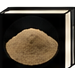
\includegraphics[width=.90cm,height=.64cm]{assets/sand_1.png}};
}

\begin{document}
\begin{tikzpicture}[x=1cm,y=1cm]
\path[use as bounding box](-.1,1.35)rectangle(19.6,13.35);
\fill[white](-.1,1.35)rectangle(19.6,13.35);

% Main title: the two-line block follows the reference's width and line spacing.
\node[font=\headingfont\bfseries\fontsize{12.8}{14.2}\selectfont]at(9.75,13.07)
  {Anchor--Canvas Surface Fusion for Aperture-Limited Sand Reconstruction};
\node[font=\headingfont\bfseries\fontsize{12.8}{14.2}\selectfont]at(9.75,12.56)
  {with a Frozen Geometry Foundation Model};

% Aperture-limited input.
\node[panel=orange,minimum width=5.00cm,minimum height=3.15cm,anchor=north west](input)at(.20,12.05){};
\person{.30}{11.73}{person_input_magnifier.png}
\node[outertitle,text=orange,anchor=north]at(2.70,11.88){Aperture-limited stream};
\node[body]at(2.70,11.17){Rotating aperture};
\sandthumb{.50}{10.30}\sandthumb{1.58}{10.30}\sandthumb{2.66}{10.30}\sandthumb{4.02}{10.30}
\node[font=\large]at(3.72,10.62){$\cdots$};
\node[body,anchor=north west,align=left,text width=4.15cm]at(.55,10.08)
  {$\bullet$ RGB frames\\[.5mm]$\bullet$ optional depth / camera hints\\[.5mm]$\bullet$ uncalibrated views};

% Change-aware streaming. The hot/cold area is deliberately close to the card height in the reference.
\node[panel=orange,minimum width=4.95cm,minimum height=3.90cm,anchor=north west](stream)at(.20,8.50){};
\person{.30}{8.18}{person_stream_warning.png}
\node[outertitle,text=orange,anchor=north]at(2.675,8.33){Change-aware streaming};
\foreach \id/\x/\ttl/\asset in {
  ch/.48/{Change\\detection}/stream_change.png,
  aw/1.98/{Bucketed\\\mbox{active window}}/stream_window.png,
  kf/3.48/{Protected\\keyframes}/stream_key.png}{
  \node[card,minimum width=1.35cm,minimum height=1.38cm,anchor=north west](\id)at(\x,7.72){};
  \node[font=\bfseries\fontsize{5.1}{5.9}\selectfont,align=center,anchor=north,text width=1.24cm]
    at($(\id.north)+(0,-.11)$){\ttl};
  \node[inner sep=0pt]at($(\id.south)+(0,.27)$){\includegraphics[width=.76cm,height=.48cm]{assets/\asset}};
}
\node[draw=green,rounded corners=3pt,line width=.7pt,fill=green!4,minimum width=4.39cm,minimum height=1.25cm,anchor=north](mem)at(2.675,6.15){};
\node[font=\bfseries\fontsize{7.2}{8.0}\selectfont,text=green,anchor=north]at($(mem.north)+(0,-.04)$){Hybrid hot/cold map};
\node[font=\bodyfont\fontsize{4.6}{5.8}\selectfont,anchor=north,align=center]at(1.42,5.79){Hot memory\\(surfel + TSDF)};
\node[font=\bodyfont\fontsize{4.6}{5.8}\selectfont,anchor=north,align=center]at(3.92,5.79){Cold storage\\(memmap)};
\node[inner sep=0pt]at(1.42,5.10){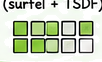
\includegraphics[width=.70cm,height=.30cm]{assets/memory_grid.png}};
\node[inner sep=0pt]at(2.675,5.13){
\includegraphics[width=.40cm,height=.46cm]{assets/memory_snow.png}};
\node[inner sep=0pt]at(3.92,5.10){
\includegraphics[width=.31cm,height=.34cm]{assets/memory_store.png}};

% Frozen geometry backend.
\node[panel=blue,minimum width=9.00cm,minimum height=3.15cm,anchor=north west](back)at(5.70,12.05){};
\person{5.80}{11.73}{person_backend_shield.png}
\node[font=\headingfont\bfseries\fontsize{8.2}{9.2}\selectfont,align=center,text=blue,anchor=north]at(10.20,11.88)
  {Frozen geometry foundation model (OmniVGGT) $\ast$};
\node[card,minimum width=2.60cm,minimum height=2.15cm,anchor=north west](mv)at(6.02,11.22){};
\node[paneltitle,anchor=north]at($(mv.north)+(0,-.08)$){Multi-view\\inputs};
\node[inner sep=0pt]at(7.32,9.80){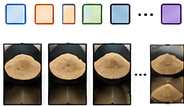
\includegraphics[width=2.02cm,height=1.03cm]{assets/mv_visual.png}};
\node[card,draw=blue,minimum width=1.84cm,minimum height=1.50cm,text width=1.62cm,
      font=\bfseries\fontsize{8}{9}\selectfont,text=blue](omni)at(9.92,10.15)
  {OmniVGGT\\[-1mm]\fontsize{6.4}{7}\selectfont(frozen)};
\node[card,minimum width=2.95cm,minimum height=2.20cm,anchor=north west](pred)at(11.34,11.22){};
\node[paneltitle,anchor=north]at($(pred.north)+(0,-.08)$){Per-frame outputs};
\foreach \yy/\asset/\label in {
  10.55/pred_depth.png/Depth map,
  10.21/pred_conf.png/Confidence,
  9.87/pred_points.png/Point map,
  9.53/pred_camera.png/Camera (rel.)}{
  \node[inner sep=0pt]at(11.76,\yy){\includegraphics[width=.34cm,height=.28cm,keepaspectratio]{assets/\asset}};
  \node[body,anchor=west]at(12.02,\yy){\label};
}
\draw[flow](mv.east)--(omni.west);
\draw[flow](omni.east)--(pred.west);

% Aperture-specific pipeline: equal cards, equal gaps, and a fixed title/image/note rhythm.
\node[panel=green,minimum width=9.35cm,minimum height=3.50cm,anchor=north west](pipe)at(5.55,8.10){};
\person{5.65}{7.78}{person_pipeline_idea.png}
\node[outertitle,text=green,anchor=north]at(10.225,7.93)
  {Aperture-specific anchor--canvas pipeline};
\foreach \id/\x/\ttl/\out in {
  h/5.855/{H-matrix\\alignment}/{\shortstack[c]{Canonical 2-D\\anchor canvas}},
  d/7.635/{Overlap depth\\correction}/{\shortstack[c]{Align scales in\\overlap regions}},
  f/9.415/{Support-aware\\fusion}/{\shortstack[c]{Single height\\per cell}},
  ho/11.195/{Hole handling\\boundary trim}/{\shortstack[c]{Remove unreliable\\rim support}},
  p/12.975/{Plane residual\\export}/{\shortstack[c]{Detrend \& export\\residuals}}}{
  \node[card,minimum width=1.62cm,minimum height=2.55cm,anchor=north west](\id)at(\x,7.38){};
  \node[font=\bfseries\fontsize{5.2}{5.9}\selectfont,align=center,text width=1.50cm,anchor=north]
    at($(\id.north)+(0,-.08)$){\ttl};
  \node[font=\fontsize{4.8}{6.8}\selectfont,align=center,anchor=south]
    at($(\id.south)+(0,.10)$){\out};
}
\node[inner sep=0pt]at(6.665,6.13){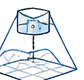
\includegraphics[width=1.14cm,height=.65cm]{assets/pipe_h.png}};
\node[inner sep=0pt]at(8.445,6.13){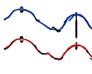
\includegraphics[width=1.14cm,height=.65cm]{assets/pipe_d.png}};
\node[inner sep=0pt]at(10.225,6.13){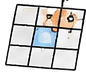
\includegraphics[width=1.14cm,height=.65cm]{assets/pipe_f.png}};
\node[inner sep=0pt]at(12.005,6.13){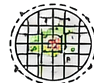
\includegraphics[width=1.14cm,height=.65cm]{assets/pipe_hole.png}};
\node[inner sep=0pt]at(13.785,6.13){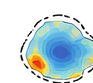
\includegraphics[width=1.14cm,height=.65cm]{assets/pipe_residual.png}};
\draw[flow](h.east)--(d.west);\draw[flow](d.east)--(f.west);
\draw[flow](f.east)--(ho.west);\draw[flow](ho.east)--(p.west);

% Outputs: narrower outer frame and taller, reference-like result cards.
\node[panel=red,minimum width=3.60cm,minimum height=7.45cm,anchor=north west](out)at(15.70,12.05){};
\person{15.80}{11.73}{person_outputs_check.png}
\node[outertitle,text=red,anchor=north]at(17.50,11.88){Outputs};
\foreach \top/\ttl in {11.30/{Dense fused surface\\[-.2mm]\fontsize{5.8}{6.4}\selectfont(point cloud)},9.65/{Height field\\[-.2mm]\fontsize{5.8}{6.4}\selectfont(anchor canvas)},8.00/{Plane residual map},6.35/{Quality metrics}}{
  \node[card,minimum width=3.14cm,minimum height=1.42cm,anchor=north](outcard)at(17.50,\top){};
  \node[cardtitle,anchor=north]at(17.50,{\top-.08}){\ttl};
}
\node[inner sep=0pt]at(17.50,10.23){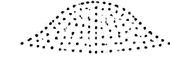
\includegraphics[width=2.02cm,height=.50cm]{assets/out_points.png}};
\node[inner sep=0pt]at(17.50,8.60){
\includegraphics[width=2.24cm,height=.58cm]{assets/out_height.png}};
\node[inner sep=0pt]at(17.50,6.95){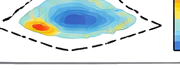
\includegraphics[width=2.18cm,height=.56cm]{assets/out_residual.png}};
\node[inner sep=0pt]at(17.02,5.30){
\includegraphics[width=.52cm,height=.46cm]{assets/out_quality_check.png}};
\node[inner sep=0pt]at(17.98,5.30){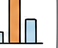
\includegraphics[width=.62cm,height=.48cm]{assets/out_quality_bars.png}};

% Bottom row.
\node[panel=orange,minimum width=4.50cm,minimum height=2.65cm,anchor=north west](scene)at(.20,4.20){};
\person{.30}{3.88}{person_scene_thinking.png}
\node[outertitle,text=orange,anchor=north]at(2.45,4.03){Target scene};
\node[inner sep=0pt]at(1.18,2.64){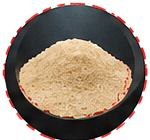
\includegraphics[width=1.65cm,height=1.40cm]{assets/target_sand_clean.png}};
\node[font=\bfseries\fontsize{4.8}{11.5}\selectfont,text width=2.45cm,anchor=north west,align=left]at(2.03,3.39)
  {$\bullet$ \mbox{Sand surface}\\$\bullet$ \mbox{Rotating aperture}\\$\bullet$ \mbox{Uncalibrated cameras}\\$\bullet$ \mbox{Boundary + aperture edge}};

\node[panel=blue,minimum width=5.30cm,minimum height=2.65cm,anchor=north west](why)at(5.15,4.20){};
\person{5.25}{3.88}{person_why_question.png}
\node[outertitle,text=blue,anchor=north]at(7.80,4.03){Why our system?};
\node[card,draw=red,minimum width=2.20cm,minimum height=1.55cm,anchor=north west]at(5.43,3.43){};
\node[font=\bfseries\fontsize{5.7}{6.4}\selectfont,text=red,anchor=north]at(6.53,3.35){Challenges};
\node[font=\fontsize{5.3}{7.0}\selectfont,text width=1.88cm,anchor=north west,align=left]at(5.60,3.03)
  {$\times$ Depth scale drift\\$\times$ Vertical ghosting\\$\times$ Seams and holes};
\node[card,draw=blue,minimum width=2.48cm,minimum height=1.55cm,anchor=north west]at(7.78,3.43){};
\node[font=\bfseries\fontsize{5.7}{6.4}\selectfont,text=blue,anchor=north]at(9.02,3.35){Our solution};
\node[font=\fontsize{5.3}{7.0}\selectfont,text width=2.02cm,anchor=north west,align=left]at(7.98,3.03)
  {\makebox[.24cm][l]{\textcolor{blue}{$\surd$}}streaming\\\makebox[.24cm][l]{\textcolor{blue}{$\surd$}}anchor alignment\\\makebox[.24cm][l]{\textcolor{blue}{$\surd$}}support fusion};

\node[panel=blue,minimum width=8.50cm,minimum height=2.65cm,anchor=north west](case)at(10.90,4.20){};
\person{11.00}{3.88}{person_case_clipboard.png}
\node[outertitle,text=blue,anchor=north]at(15.15,4.03){Case study (12 frames)};
\foreach \x in {12.57,14.25,15.93,17.61}{\draw[ink!45,line width=.45pt](\x,3.40)--(\x,1.72);}
\node[inner sep=0pt]at(11.74,3.18){
\includegraphics[width=.86cm,height=.62cm,keepaspectratio]{assets/case_key.png}};
\node[inner sep=0pt]at(13.41,3.18){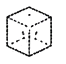
\includegraphics[width=.82cm,height=.64cm,keepaspectratio]{assets/case_cube.png}};
\node[inner sep=0pt]at(15.09,3.18){
\includegraphics[width=.80cm,height=.64cm,keepaspectratio]{assets/case_grid.png}};
\node[inner sep=0pt]at(16.77,3.18){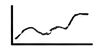
\includegraphics[width=1.05cm,height=.56cm,keepaspectratio]{assets/case_residual.png}};
\node[inner sep=0pt]at(18.45,3.18){
\includegraphics[width=.78cm,height=.68cm,keepaspectratio]{assets/case_stopwatch.png}};
\foreach \x/\label/\value/\tone in {
  11.74/Keyframes/3/blue,
  13.41/Points/{440,911}/blue,
  15.09/{Internal holes}/0/blue,
  16.77/{Depth residual}/{0.0278 $\rightarrow$\\0.0030}/green,
  18.45/{Streaming speed}/{0.973 s}/green}{
  \node[tinybody,text width=1.38cm,anchor=north]at(\x,2.79){\label};
  \node[font=\bfseries\fontsize{8}{9}\selectfont,text=\tone,align=center,anchor=north]at(\x,2.35){\value};
}

% Inter-panel data and control flow. All arrow shafts occupy the explicit gaps between frames.
\draw[outerflow](input.east)--(back.west);
\draw[outerflow](2.70,8.90)--(2.70,8.50);
\draw[outerflow](5.15,6.35)--(5.55,6.35);
\draw[outerflow](10.20,8.90)--(10.20,8.10);
\draw[outerflow](14.90,6.35)--(15.70,6.35);
\draw[outerflow](10.225,4.60)--(10.225,4.38)-|(2.70,4.60);
\draw[outerflow](scene.east)--(why.west);
\draw[outerflow](why.east)--(case.west);
\draw[aux](14.70,10.47)--(15.46,10.47)--(15.46,7.00)--(14.90,7.00);

\rim{input}{orange}\rim{stream}{orange}\rim{back}{blue}\rim{pipe}{green}
\rim{out}{red}\rim{scene}{orange}\rim{why}{blue}\rim{case}{blue}
\end{tikzpicture}
\end{document}
